\chapter{Historical Models of Image Generation}

In this chapter, I aim to provide an overview of three important generative modeling techniques: Noise Contrastive Estimation (NCE), Variational Autoencoders (VAEs), and Diffusion Models. These models have each played a significant role in the evolution of generative modeling and continue to influence modern approaches in the field. 

\section{Noise Contrastive Estimation (NCEs)}

Noise Contrastive Estimation (NCE) was introduced in 2010 by Gutmann and Hyvärinen as a method for estimating parameters in unnormalized probabilistic models. It offers an efficient alternative to Maximum Likelihood Estimation (MLE), particularly in cases where MLE can become computationally expensive, especially with large-scale models. NCE reframes the challenge of normalizing probability distributions into a more manageable binary classification problem \citep{10.48550/arxiv.1711.00658}. 

The core idea behind NCE is to treat MLE as a binary classification task. Traditionally, training models for unnormalized probability distributions using MLE involves calculating the partition function, which can be computationally infeasible for large datasets. NCE mitigates this difficulty by incorporating noise samples drawn from a known distribution. The model is then trained to differentiate between real data and noise samples, with higher probabilities assigned to real data and lower probabilities to noise. This approach allows the model to learn the data distribution without the need for explicit normalization \citep{10.48550/arxiv.2110.11271}.

\subsection{NCE Architecture}
In NCE, the likelihood of a data point \( x \) is reformulated as the probability that it comes from the real data distribution rather than from the noise distribution. As depicted in Figure~\ref{fig:NCE_structure}, the architecture of a typical NCE model includes an input layer, a hidden layer, and an output layer. The input layer receives both real and noise samples, while the hidden layer learns representations of these samples. The output layer functions as a binary classifier, producing probabilities that indicate whether a given sample is real or noise.

\begin{figure}[H]
    \centering
    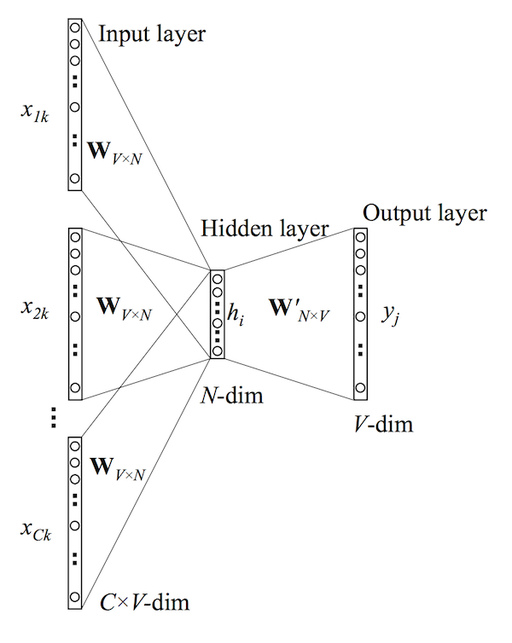
\includegraphics[width=0.9\textwidth]{./Images/NCE_structure.jpg}
    \caption{NCE Architecture.}
    \label{fig:NCE_structure}
\end{figure}

\begin{itemize}
    \item \textbf{Data and Noise Samples}: NCE introduces noise samples from a known distribution to compare with actual data. These noise samples act as negative examples in the classification task, while the real data serves as positive examples \citep{10.48550/arxiv.1711.00658}.
    \item \textbf{Binary Classification}: The task of differentiating between real and noise samples is framed as a binary classification problem, which can be optimized using standard logistic regression techniques \citep{10.18653/v1/e17-2003}.
\end{itemize}

\subsection{NCE Objective Function}
In NCE, the probability \( P(y = 1 | x) \), where \( y = 1 \) indicates that \( x \) is a real sample, is defined as:

\begin{equation}
P(y = 1 | x) = \frac{p_{\theta}(x)}{p_{\theta}(x) + k p_{\text{noise}}(x)}
\end{equation}

Where \( p_{\theta}(x) \) is the unnormalized probability assigned to the sample \( x \) by the model, \( p_{\text{noise}}(x) \) is the probability assigned to the noise sample, and \( k \) is the ratio of noise samples to real samples.

The corresponding probability that a sample \( x \) is from the noise distribution is given by:

\begin{equation}
P(y = 0 | x) = \frac{k p_{\text{noise}}(x)}{p_{\theta}(x) + k p_{\text{noise}}(x)}
\end{equation}

The NCE objective then seeks to maximize the log-probabilities of correctly classifying real and noise samples:

\begin{equation}
\mathcal{L}_{NCE} = \sum_{i=1}^{N} \left[ \log P(y=1 | x_i) + \sum_{j=1}^{k} \log P(y=0 | x_j) \right]
\end{equation}

This method circumvents the need for computing the partition function, which is typically required in Maximum Likelihood Estimation (MLE), making NCE particularly useful for large-scale models \citep{10.48550/arxiv.2110.11271}.
\subsection{Comparison with GANs}

Noise Contrastive Estimation (NCE) and Generative Adversarial Networks (GANs) are both prominent methods in generative modeling, but they take different approaches to training and model estimation.

\begin{itemize}
    \item \textbf{Training Stability}: One of NCE’s key advantages over GANs is the stability it provides during training. GANs frequently suffer from challenges such as mode collapse and instability due to the adversarial nature of the training process, where the generator and discriminator are pitted against each other. NCE, by contrast, frames the training process as a straightforward binary classification task, which tends to be more stable and can be optimized with logistic regression \citep{10.18653/v1/e17-2003}.
    
    \item \textbf{Computational Efficiency}: Training GANs requires simultaneously optimizing two models—the generator and the discriminator—which can lead to higher computational costs, particularly when tuning their interactions for better performance. NCE, on the other hand, simplifies the problem by reducing it to a comparison between real data and noise samples, avoiding the adversarial framework and offering a more computationally efficient solution, especially for large-scale models \citep{10.21437/interspeech.2016-1295}.
    
    \item \textbf{Handling Unnormalized Models}: NCE is particularly suited for training unnormalized probabilistic models, where computing the partition function is impractical or impossible. GANs, however, are focused on generating realistic samples and, while they do not require explicit normalization, they do not address the problem of unnormalized models as directly as NCE does \citep{10.48550/arxiv.2101.03288}.
    
    \item \textbf{Model Interpretability}: In NCE, the model explicitly learns to estimate the probability of real data versus noise, providing insights into the data distribution. In comparison, GANs focus on generating realistic samples without explicitly modeling probabilities, which can make their internal latent space less interpretable than that of NCE-based models.
    
    \item \textbf{Applications in Language Models and Word Embeddings}: NCE is particularly beneficial in tasks such as word embeddings and large-scale language models, where normalizing the likelihood function over vast vocabularies is computationally prohibitive. GANs have been applied in text generation, but NCE’s efficiency in handling large-scale vocabulary models makes it more suitable for these problems \citep{10.48550/arxiv.2101.03288}.
\end{itemize}

\subsection{Applications of NCE}

NCE is highly effective in a variety of machine learning tasks, particularly those that involve large datasets and unnormalized models:
\begin{itemize}
    \item \textbf{Word Embeddings}: NCE is widely used in training word embeddings, where the size of the vocabulary makes normalization computationally infeasible.
    \item \textbf{Language Models}: Beyond word embeddings, NCE has been applied to training large-scale language models, where traditional likelihood-based methods may become computationally expensive.
    \item \textbf{Energy-Based Models}: NCE is also effective in training energy-based models, which typically require an intractable partition function for normalization.
\end{itemize}

NCE allows models to scale efficiently, making it an invaluable tool in areas ranging from natural language processing to computer vision.

\subsection{Limitations of NCE}

While NCE has proven to be a powerful estimation technique, it is not without limitations. A key challenge lies in selecting an appropriate noise distribution. Poor choices in this regard can lead to suboptimal parameter estimates and slower convergence during training \citep{10.48550/arxiv.2110.11271}.

\begin{itemize}
    \item \textbf{Noise Distribution Sensitivity}: The success of NCE relies heavily on choosing a noise distribution that is sufficiently different from the real data distribution. If the noise distribution is poorly chosen, the model may struggle to differentiate between real and noise samples \citep{10.48550/arxiv.2110.11271}.
    \item \textbf{Handling Complex Data Distributions}: NCE may encounter difficulties with highly complex data distributions, particularly in cases where defining an appropriate noise distribution is challenging \citep{10.48550/arxiv.2110.11271}.
\end{itemize}


\section{Variational Autoencoders (VAEs)}

Variational Autoencoders (VAEs), introduced in 2013, represent one of the foundational approaches to generative modeling. The primary goal of VAEs is to model the underlying distribution of data by learning a compressed latent representation, denoted as \(z\), from the input data \(x\).

\subsection{VAE Architecture}
VAEs consist of two main components: an encoder and a decoder. The encoder maps input data into a latent space, where the latent variables are generally assumed to follow a Gaussian distribution. This assumption simplifies the training process and enables techniques such as the reparameterization trick, which facilitates backpropagation through stochastic layers \citep{10.1561/2200000056}. The decoder then reconstructs the input data from the latent variables, ensuring that the essential characteristics of the data distribution are captured.

As illustrated in Figure~\ref{fig:VAE_structure}, the VAE architecture comprises:
\begin{itemize}
    \item \textbf{Encoder}: The encoder takes the input data \(x\) and compresses it into a latent representation \(z\). The latent variables are sampled from a Gaussian distribution, which aids in simplifying the optimization process.
    \item \textbf{Decoder}: The decoder reconstructs the original data \(x'\) from the latent representation \(z\), aiming to produce data that closely resembles the input.
\end{itemize}

\begin{figure}[H]
    \centering
    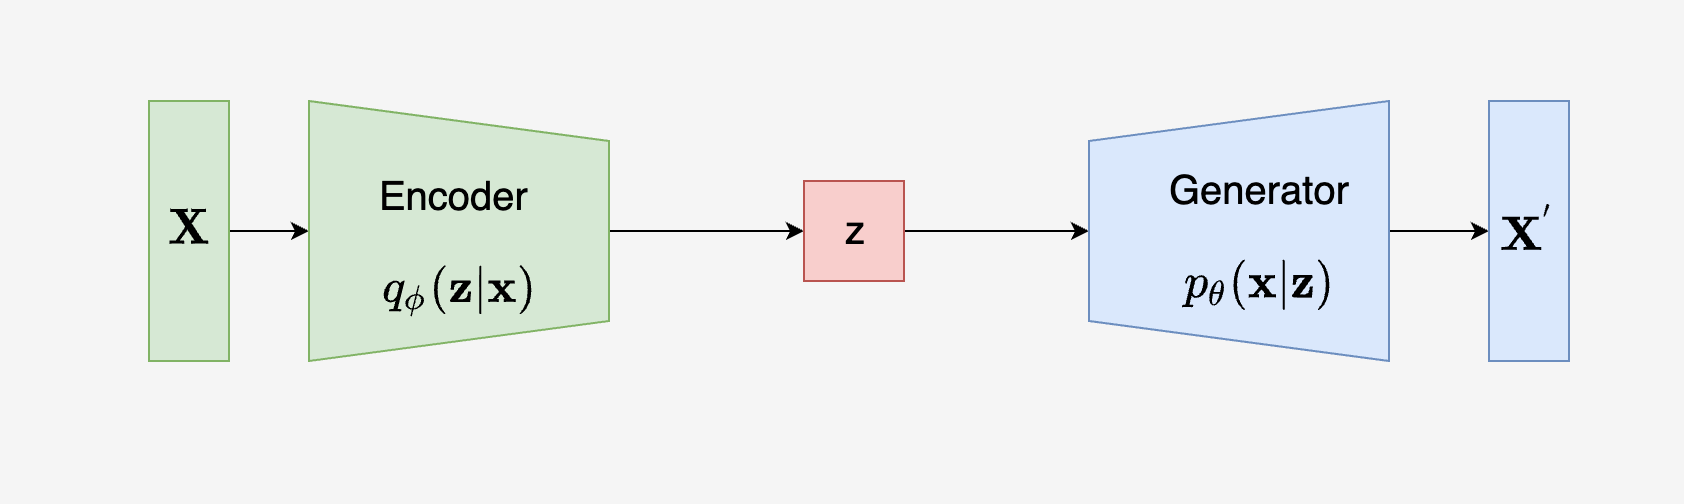
\includegraphics[width=0.9\textwidth]{./Images/VAE_structure.jpg}
    \caption{VAE Architecture.}
    \label{fig:VAE_structure}
\end{figure}

\subsection{VAE Objective Function}
The VAE loss function is designed to balance two objectives: accurate data reconstruction and regularization of the latent space. The total loss combines a reconstruction loss with a Kullback-Leibler (KL) divergence term, which helps the model learn a smooth, continuous representation of the latent space \citep{10.3390/jimaging4020036}.

The VAE aims to maximize the variational lower bound, encouraging both accurate reconstruction and a well-structured latent space. This, in turn, enables the model to generate new data by sampling from the latent space and reconstructing it using the decoder.

The loss function of a VAE is expressed as follows:

\begin{equation}
\mathcal{L} = \mathbb{E}_{q_\phi(z|x)}[\log p_\theta(x|z)] - D_{KL}(q_\phi(z|x) \| p(z))
\end{equation}

Where:
\begin{itemize}
    \item \(\mathcal{L}\): The total loss that the model seeks to minimize.
    \item \(\mathbb{E}_{q_\phi(z|x)}[\log p_\theta(x|z)]\): This term represents the expected log-likelihood of the reconstructed data \(x'\) given the latent variable \(z\). The distribution \(q_\phi(z|x)\) corresponds to the encoder's approximation of the posterior, while \(p_\theta(x|z)\) represents the decoder's likelihood of reconstructing the input data.
    \item \(D_{KL}(q_\phi(z|x) \| p(z))\): The KL divergence measures the difference between the encoder's learned latent distribution \(q_\phi(z|x)\) and the prior distribution \(p(z)\), which is typically Gaussian.
\end{itemize}

\subsection{Comparison with GANs}

When compared to Generative Adversarial Networks (GANs), VAEs exhibit several advantages. One of the most notable strengths of VAEs is their training stability. In contrast to GANs, which involve training both a generator and a discriminator—a process that can lead to issues such as mode collapse—VAEs have a single objective function. This objective combines reconstruction loss and KL divergence, making the training process more straightforward and less prone to instability \citep{10.1561/2200000056}.

Another key strength of VAEs is their ability to generate smooth transitions between data points. This capability is particularly valuable for applications that require meaningful interpolation in the latent space, such as image generation, anomaly detection, and data imputation \citep{10.1088/2632-2153/ab80b7}\citep{10.48550/arxiv.2002.10464}. GANs, on the other hand, do not explicitly model the latent space, which can limit their interpretability and flexibility in certain tasks.

However, GANs are often favored for generating sharper and more realistic images, particularly in high-resolution tasks. The adversarial loss in GANs encourages the generator to produce outputs that closely resemble real data, while VAEs, due to their reliance on Gaussian priors, tend to generate slightly blurrier images \citep{10.1109/access.2020.2977671}. Nonetheless, VAEs offer greater flexibility and scalability, as they can be trained using standard gradient descent methods and do not require the complex adversarial framework inherent to GANs.

\subsection{Applications of VAEs}

The versatility of VAEs extends to a wide range of applications, many of which benefit from the structured latent space that VAEs provide:
\begin{itemize}
    \item \textbf{Image Generation}: VAEs can generate new images by sampling from the latent space and decoding the latent vectors into realistic image representations.
    \item \textbf{Anomaly Detection}: VAEs are often used to identify outliers in data by examining reconstruction errors. Data points with high reconstruction loss may be flagged as anomalies.
    \item \textbf{Data Imputation}: VAEs are capable of filling in missing data by reconstructing the incomplete data from latent representations, making them useful for handling datasets with gaps or missing values.
\end{itemize}

\subsection{Limitations of VAEs}

While VAEs have proven effective in many applications, they also have certain limitations:
\begin{itemize}
    \item \textbf{Blurred Outputs}: Due to the Gaussian prior assumption in the latent space, VAEs often generate blurrier outputs compared to GANs, which may affect performance in tasks requiring high-resolution and sharp images \citep{10.1109/access.2020.2977671}.
    \item \textbf{Difficulty with Discrete Data}: VAEs struggle to effectively model discrete data, as backpropagation through continuous latent variables is not well-suited to handle discrete structures \citep{10.48550/arxiv.1909.13062}.
    \item \textbf{Limited Diversity}: VAEs may not capture the full complexity and diversity of the data distribution as effectively as GANs, particularly when generating high-resolution images \citep{10.48550/arxiv.2106.06500}.
\end{itemize}

\section{Diffusion Models}

Diffusion models, emerging in the early 2020s, represent a significant advancement in generative modeling. These models progressively add noise to data and then learn to reverse this process, effectively "denoising" it back to its original form. This iterative process distinguishes diffusion models from traditional approaches like GANs and VAEs \citep{10.48550/arxiv.2105.05233}.

\subsection{Diffusion Model Architecture}

The core idea behind diffusion models relies on a Markov chain where noise is added in the forward process, starting from a simple distribution (e.g., Gaussian), and reversed through a learned denoising mechanism \citep{10.48550/arxiv.2009.09761}, \citep{10.48550/arxiv.2206.05564}. This approach has proven effective in generating high-quality samples across various domains, such as image synthesis, audio generation, and medical imaging \citep{10.48550/arxiv.2201.11972}, \citep{10.48550/arxiv.2211.00611}. In several benchmarks, diffusion models have outperformed GANs \citep{10.48550/arxiv.2105.05233}, \citep{10.48550/arxiv.2201.00308}.

The process involves two key steps, as shown in Figure~\ref{fig:Diffusion_structure}:
\begin{itemize}
  \item \textbf{Forward Process}: Gradually adds Gaussian noise to data \(x_0\), creating noisy versions of the data \(x_1, x_2, \dots, x_T\). Each step increases the noise level, leading to a completely noisy version \(z\).
  \item \textbf{Reverse Process}: The model learns to reverse the noise addition process, starting from the fully noisy version \(z\), and progressively denoising it to recover data that resembles the original input \(x_0\).
\end{itemize}

\begin{figure}[H]
    \centering
    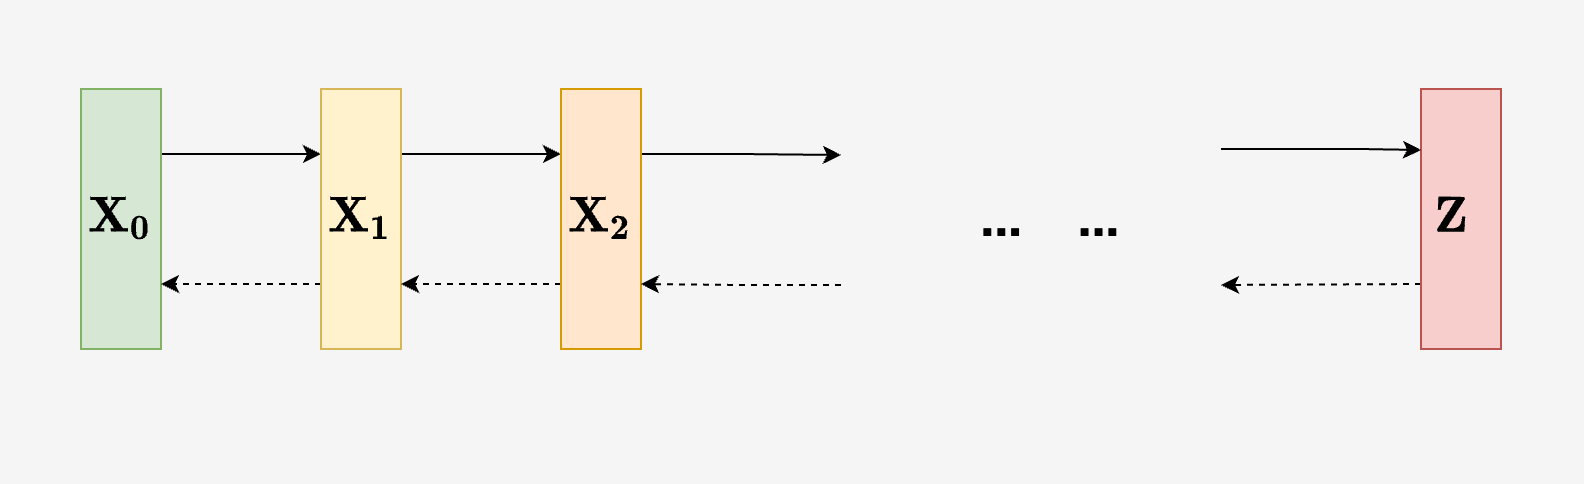
\includegraphics[width=0.9\textwidth]{./Images/Diffusion_structure.jpg}
    \caption{Diffusion Model Architecture.}
    \label{fig:Diffusion_structure}
\end{figure}

\subsection{Diffusion Model Objective Function}

The training objective for diffusion models is to minimize the difference between the real data distribution and the distribution of generated data across all time steps:

\begin{equation}
L = \sum_{t=1}^{T} \mathbb{E}_{x_0, \epsilon} \left[ \|\epsilon - \epsilon_\theta(x_t, t)\|^2 \right]
\end{equation}

Where:
\begin{itemize}
    \item \(L\): The loss function to be minimized.
    \item \(T\): The total number of time steps in the diffusion process.
    \item \(x_0\): The original data sample.
    \item \(x_t\): The data at time step \(t\), after adding noise.
    \item \(\epsilon\): The noise added to the data at each step.
    \item \(\epsilon_\theta(x_t, t)\): The model's estimate of the noise at time step \(t\).
\end{itemize}

\subsection{Comparison with GANs}

Diffusion models and Generative Adversarial Networks (GANs) represent two distinct approaches in generative modeling, each with its strengths and weaknesses. A key advantage of diffusion models is their training stability. Unlike GANs, which often suffer from unstable dynamics due to the adversarial competition between the generator and discriminator, diffusion models follow a simpler, noise-reversal process that avoids these issues \citep{10.1109/access.2023.3272032}. This stability helps diffusion models avoid problems like mode collapse, where GANs fail to capture the diversity of the data distribution \citep{10.1049/ipr2.12487}, \citep{10.3390/e25121657}.

Diffusion models also excel in generating diverse, high-quality samples through a gradual denoising process, allowing for controlled generation \citep{10.1117/1.jei.32.4.043029}. In contrast, GANs tend to produce sharper but less diverse images, often overfitting to specific modes of the data \citep{10.48550/arxiv.1910.04302}, \citep{10.48550/arxiv.2207.01561}. This trade-off between sharpness and diversity is a known limitation of GANs \citep{10.1111/rssb.12476}.

However, GANs remain preferred for tasks requiring extremely high-resolution and photorealistic images, such as human face generation, where they outperform diffusion models in terms of detail and realism \citep{10.54254/2755-2721/18/20230984}, \citep{10.3390/e22091055}.

\subsection{Applications of Diffusion Models}

Diffusion models have found a wide range of applications, especially in fields where stability and quality of generation are important. Some notable applications include:
\begin{itemize}
    \item \textbf{Image Generation}: Diffusion models have proven effective in generating photorealistic images, similar to GANs, but with more stable training dynamics. Recent innovations, such as classifier-free guidance, have further enhanced the quality of generated samples by allowing the model to generate data without relying on an explicit classifier \citep{10.48550/arxiv.2207.12598}.
    \item \textbf{Text-to-Image Generation}: Advancements in diffusion models have also been applied to text-to-image synthesis, where a text prompt is converted into a corresponding image. These models can produce diverse outputs based on input descriptions. Additionally, techniques like Denoising Diffusion Implicit Models (DDIMs) have accelerated the sampling process, making diffusion models more practical for real-time applications \citep{10.48550/arxiv.2010.02502}, \citep{10.48550/arxiv.2111.15640}.
    \item \textbf{Speech Synthesis}: Diffusion models have been applied to generating high-quality audio data. For example, they are used in text-to-speech systems to generate realistic human speech. These models have demonstrated remarkable performance in generating high-fidelity audio outputs \citep{10.48550/arxiv.2201.11972}, \citep{10.48550/arxiv.2009.09761}.
    \item \textbf{Anomaly Detection and Medical Imaging}: Similar to VAEs, diffusion models can be used to detect anomalies by evaluating how well a noisy sample can be denoised. Poor reconstructions may indicate that the input is anomalous or different from the training data. Diffusion models have also been applied in medical image segmentation tasks, such as the MedSegDiff model, which enhances segmentation by leveraging diffusion processes \citep{10.48550/arxiv.2211.00611}. These models have shown their ability to handle complex data structures, proving their versatility across different domains.
\end{itemize}

Recent innovations in diffusion models have further enhanced their applicability and efficiency. By reducing the computational burden associated with the iterative sampling process, models like DDIMs maintain the generative capabilities of traditional diffusion models while improving their practicality for real-time applications \citep{10.48550/arxiv.2101.02388}.

\subsection{Limitations of Diffusion Models}

Despite the significant advancements that diffusion models have brought to generative modeling, they are not without limitations, which can be categorized into three primary areas: computational intensity, generation speed, and sample sharpness.

\begin{itemize}
    \item \textbf{Computationally Intensive}: Diffusion models are computationally expensive due to their iterative nature, which involves progressively adding and removing noise from data. This process requires significantly more computational resources compared to GANs, which generate data in a single forward pass through the generator \citep{10.1109/msp.2017.2765202}, \citep{10.1145/3422622}. This computational burden can limit their practical use, especially in scenarios requiring rapid generation \citep{10.48550/arxiv.2211.07804}.
    
    \item \textbf{Generation Speed}: Diffusion models are slower than GANs in terms of sample generation. Producing a single sample often requires hundreds or even thousands of time steps, significantly increasing the generation time compared to the near-instantaneous output of GANs \citep{10.48550/arxiv.2011.13456}, \citep{10.48550/arxiv.2010.02502}. This can be a critical drawback in real-time applications.
    
    \item \textbf{Sample Sharpness}: While diffusion models generate diverse outputs, they may not always match the photorealism and fine detail achieved by GANs, especially in tasks requiring intricate details \citep{10.48550/arxiv.2105.05233}, \citep{10.1109/cvpr52688.2022.01117}. This can affect their suitability for applications such as high-resolution image generation or medical imaging \citep{10.48550/arxiv.2211.07804}.
\end{itemize}
